\documentclass[12pt]{beamer}
\newenvironment{ConCodigo}[1]
  {\begin{frame}[fragile,environment=ConCodigo]{#1}}
  {\end{frame}}
\graphicspath{{Imagenes/}{../Imagenes/}}
\usepackage[utf8]{inputenc}
\usepackage[spanish]{babel}
\usepackage{hyperref}
\usepackage{etex}
%\reserveinserts{28}
\usepackage{amsmath}
\usepackage{amsthm}
\usepackage{mathtools}
\usepackage{multicol}
\usepackage{multirow}
\usepackage{tabulary}
\usepackage{booktabs}
\usepackage{nccmath}
\usepackage{physics}
\usepackage{biblatex}
\usepackage[outdir=./]{epstopdf}
%\epstopdfsetup{outdir=./}
\usepackage{graphicx}
%\usepackage{enumitem,xcolor}
\usepackage{siunitx}
%\sisetup{scientific-notation=true}
%\usepackage{fontspec}
\usepackage{lmodern}
\usepackage{float}
\usepackage[format=hang, font=footnotesize, labelformat=parens]{caption}
\usepackage[autostyle,spanish=mexican]{csquotes}
\usepackage{standalone}
\usepackage{blkarray}
\usepackage{algorithm}
\usepackage{algorithmic}
\usepackage{tikz}
\usepackage[siunitx, RPvoltages]{circuitikz}
\usetikzlibrary{arrows,patterns,shapes}
\usetikzlibrary{decorations.markings}
\usetikzlibrary{arrows}
\usepackage{color}
\usepackage{xcolor}
%\usepackage{beton}
%\usepackage{euler}
%\usepackage[T1]{fontenc}
\usepackage[sfdefault]{roboto}  %% Option 'sfdefault' only if the base font of the document is to be sans serif
\usepackage[T1]{fontenc}
\renewcommand*\familydefault{\sfdefault}
\DeclareGraphicsExtensions{.pdf,.png,.jpg}
\usepackage{hyperref}
\renewcommand {\arraystretch}{1.5}
\newcommand{\python}{\texttt{python}}
\usefonttheme[onlymath]{serif}
\setbeamertemplate{navigation symbols}{}
\usetikzlibrary{patterns}
\usetikzlibrary{decorations.markings}
\tikzstyle{every picture}+=[remember picture,baseline]
%\tikzstyle{every node}+=[inner sep=0pt,anchor=base,
%minimum width=2.2cm,align=center,text depth=.15ex,outer sep=1.5pt]
%\tikzstyle{every path}+=[thick, rounded corners]
\setbeamertemplate{caption}[numbered]
\newcommand{\ptm}{\fontfamily{ptm}\selectfont}
%Se usa la plantilla Warsaw modificada con spruce
\mode<presentation>
{
  \usetheme{Warsaw}
  \setbeamertemplate{headline}{}
  \useoutertheme{default}
  \usecolortheme{albatross}
  \setbeamercovered{invisible}
}
% \AtBeginSection[]
% {
% \begin{frame}<beamer>{Contenido}
% \normalfont\mdseries
% \tableofcontents[currentsection]
% \end{frame}
% }

\input{../Preambulos/pre_plantilla_Warsaw_spruce}
\input{../Preambulos/pre_codigo}
\makeatletter
\setbeamertemplate{footline}
%\setbeamercolor{title in head/foot}{fg=Green}
{
  \leavevmode%
  \hbox{%
  \begin{beamercolorbox}[wd=.333333\paperwidth,ht=2.25ex,dp=1ex,center]{author in head/foot}%
    \usebeamerfont{author in head/foot} \textcolor{white}{\insertsection}
  \end{beamercolorbox}}%
  \begin{beamercolorbox}[wd=.333333\paperwidth,ht=2.25ex,dp=1ex,center]{title in head/foot}%
    \usebeamerfont{title in head/foot} \textcolor{white}\insertsubsection
  \end{beamercolorbox}%
  \begin{beamercolorbox}[wd=.333333\paperwidth,ht=2.25ex,dp=1ex,right]{date in head/foot}%
    \usebeamerfont{date in head/foot} \textcolor{white}\insertshortdate{}\hspace*{2em}
    \textcolor{white}\insertframenumber{} / \textcolor{white}\inserttotalframenumber\hspace*{2ex} 
  \end{beamercolorbox}}%
  \vskip0pt%
\makeatother
\title{Técnicas de Interpolación}
\subtitle{Tema 2 - Operaciones matemáticas básicas}
\author{M. en C. Gustavo Contreras Mayén}
\date{\today}
\institute{Facultad de Ciencias - UNAM}
\titlegraphic{\includegraphics[width=1.75cm]{Imagenes/escudo-facultad-ciencias}\hspace*{4.75cm}~%
   \includegraphics[width=1.75cm]{Imagenes/escudo-unam}
}
\begin{document}
\maketitle
\fontsize{14}{14}\selectfont
\spanishdecimal{.}
\section*{Contenido}
\frame{\tableofcontents[currentsection, hideallsubsections]}
\section{Introducción}
\frame{\tableofcontents[currentsection, hideothersubsections]}
\subsection{Definición de interpolación}
\begin{frame}
\frametitle{Iniciamos}
Dados los $n+1$ pares de datos $(x_{i},y_{i})$, con $i=0,1,\ldots,n$, queremos estimar el valor de $y(x)$
\end{frame}
\begin{frame}
\frametitle{Interpolación}
Una parte importante en el trabajo del físico es la interpretación de datos experimentales o cálculos teóricos.
\end{frame}
\begin{frame}
\frametitle{Interpolación}
Normalmente cuando hacemos mediciones, tenemos un conjunto discreto de puntos que representan nuestro experimento.
\end{frame}
\begin{frame}
\frametitle{Interpolación}
Para facilitar el trabajo, suponemos que el experimento puede representarse por un par de valores: una \textit{variable independiente $x$} la cual podemos controlar y una cantidad $y$, que se mide en el punto $x$.
\end{frame}
\begin{frame}
\frametitle{Interpolación vs ajuste con curvas}
Hay una diferencia entre interpolación y el ajuste de curvas.
\\
\bigskip
En la interpolación se \emph{construye una curva a través de los puntos de datos}.
\end{frame}
\begin{frame}
\frametitle{Interpolación vs ajuste con curvas}
El ajuste de curvas se aplica a los datos que contienen una dispersión (ruido), por lo general debida a errores de medición.
\\
\bigskip
En este caso, \emph{queremos encontrar una curva suave que se aproxima a los datos en algún sentido}. De tal manera que la curva no toca necesariamente los puntos de datos.
\end{frame}
\begin{frame}[fragile]
\frametitle{Interpolación vs ajuste con curvas}

%\begin{tikzpicture}[scale=0.8]
%\draw [->] (0,0) -- (7,0) node [align = left, below] {x};
%\draw [->] (0,0) -- (0,5) node [align = left, above] {y};
%\draw (0.5,0.5)circle (0.1cm);
%\draw (2,1)circle (0.1cm);
%\draw (4.5,2.5)circle (0.1cm);
%\draw (6,4)circle (0.1cm);
%\draw (0,0) .. controls (0.3,0.3) and (0.5,0.5) .. (0.65,0.65)
%			.. controls (0.7,0.7) and (2,1) .. (6.5,4.5);
%\end{tikzpicture}
\begin{figure}
\centering
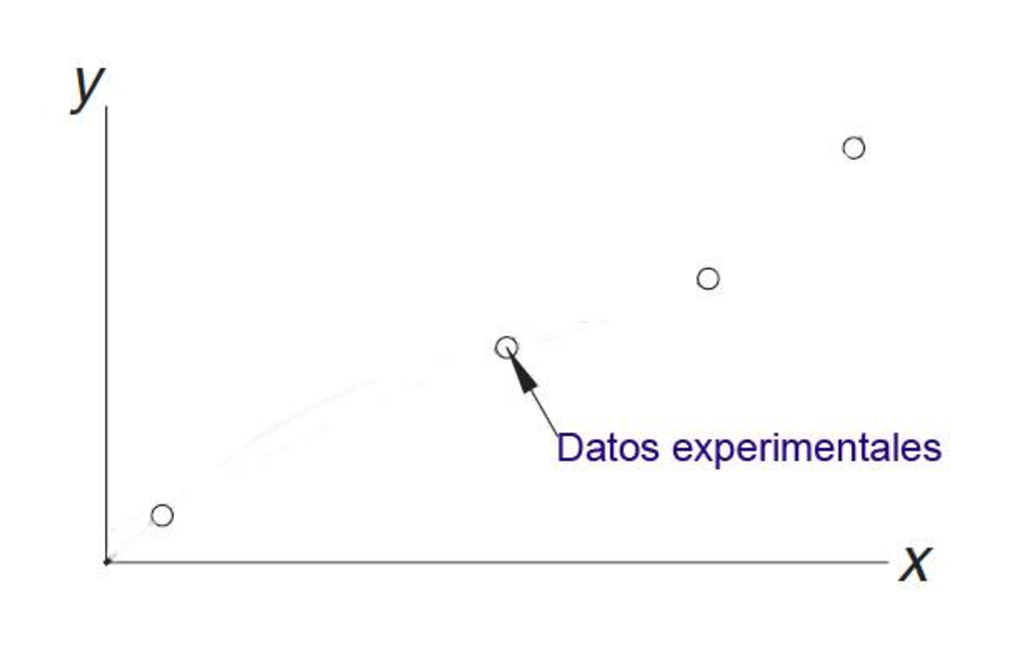
\includegraphics[scale=0.55]{Imagenes/Interpol01.eps}
\caption{Tenemos un conjunto de datos experimentales obtenidos en el laboratorio.}
\end{figure}
\end{frame}
\begin{frame}[fragile]
\frametitle{Interpolación vs ajuste con curvas}
\begin{figure}
\centering
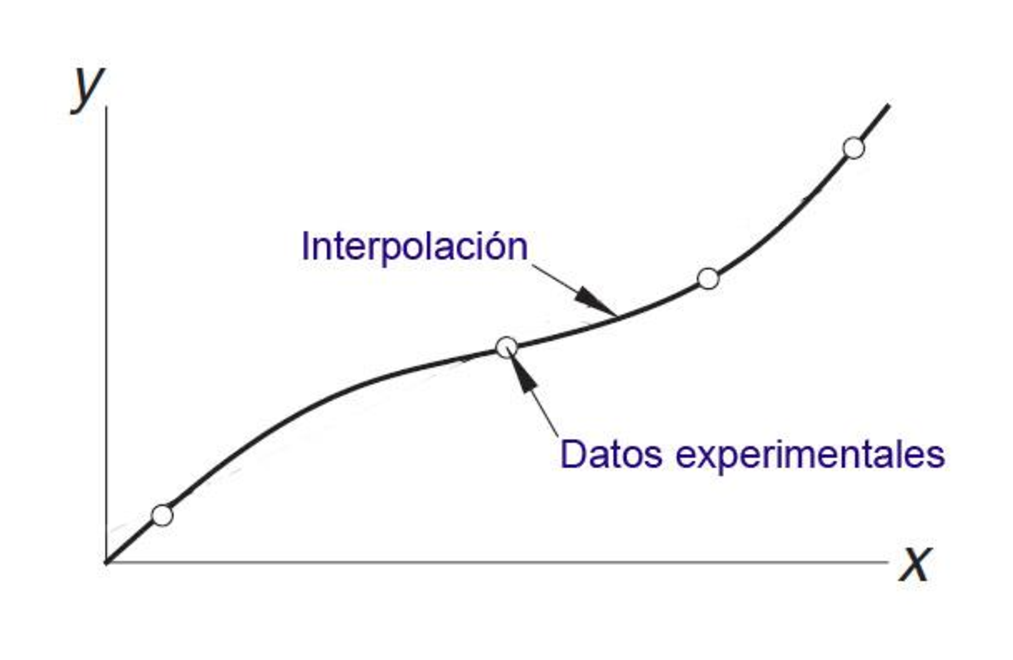
\includegraphics[scale=0.55]{Imagenes/Interpol02.eps}
\caption{Con la interpolación se construye una curva suave que \enquote{toca} a los puntos experimentales}.
\end{figure}
\end{frame}
\begin{frame}[fragile]
\frametitle{Interpolación vs ajuste con curvas}
\begin{figure}
\centering
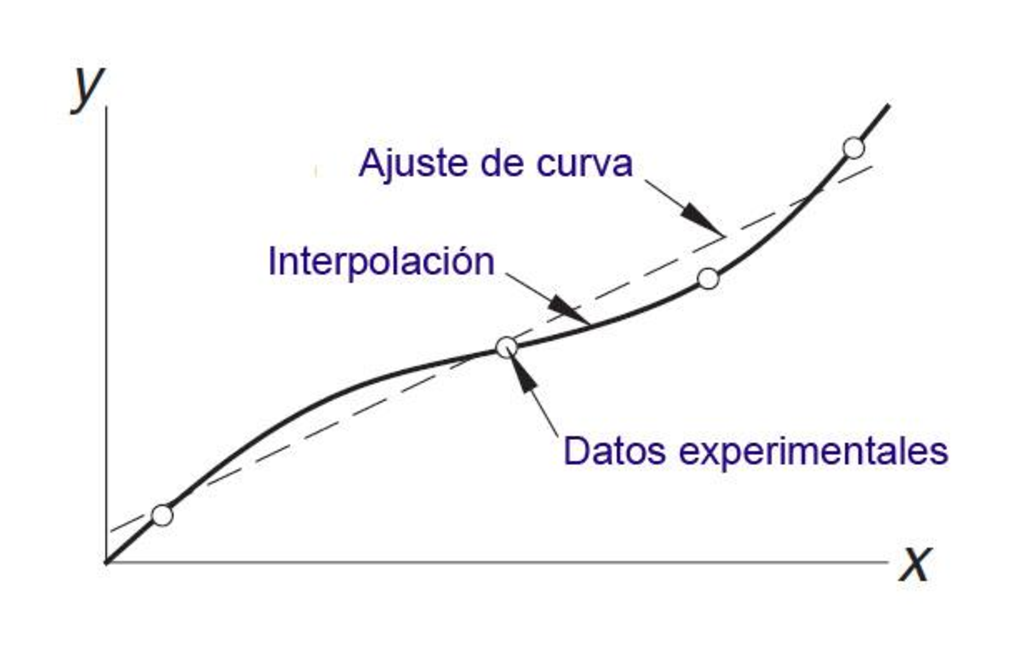
\includegraphics[scale=0.55]{Imagenes/Interpol03.eps}
\caption{La técnica de ajuste de curvas es una aproximación al conjunto de datos.}
\end{figure}
\end{frame}
\begin{frame}
\frametitle{Ejemplo}
Tomemos como ejemplo una fuente radioactiva y un detector, el cual contabiliza el número de decaimientos.
\\
\bigskip
Para determinar la vida media de la fuente, debemos de contar los decaimientos $N_{0}$, $N_{1}$, $N_{2}$, $\ldots$, $N_{k}$, en los tiempos $t_{0}$, $t_{1}$, $t_{2}$, $\ldots$, $t_{k}$
\end{frame}
\begin{frame}
\frametitle{Ejemplo}
En este ejemplo, \textcolor{red}{la variable independiente es $t$}, siendo la forma  apropiada para resolver el problema. 
\\
\bigskip
Sin embargo, tenemos un conjunto discreto de pares de números $(t_{k},N_{k})$ en el rango de $(t_{0}, t_{k}$)
\end{frame}
\begin{frame}
\frametitle{Ejemplo}
Con la intención de obtener información del experimento, deberíamos de encontrar una función analítica que nos devuelva el valor de $N$ para cualquier punto arbitrario $t$.
\end{frame}
\begin{frame}
\frametitle{Ejemplo}
Pero a veces, el tratar de encontrar una función analítica es imposible, o el pensar en utilizar una función conocida, nos podría llevar mucho tiempo para calcularla, más si nuestro interés se basa en una pequeña vecindad de la variable independiente.
\end{frame}
\begin{frame}
\frametitle{Ejemplo 2}
Supongamos que tenemos una fuente radioactiva de {}$^{241}$Am, una fuente de rayos $\alpha$. Su vida media es $\tau_{\frac{1}{2}}=430$ años.
\\
\bigskip
Obviamente no podríamos determinar su vida media midiéndola, ya que el decaimiento es lento y quizá lo que podríamos hacer es medir cada lunes durante algunos meses: después de cinco meses (por ejemplo) podríamos detener las mediciones y revisar los datos.
\end{frame}
\begin{frame}
\frametitle{Ejemplo 2}
Una pregunta que nos podemos plantear es: ¿cuál fue la actividad el miércoles de la tercera semana de mediciones? 
\\
\bigskip
Ya que ese día está dentro del rango de mediciones $(t_{0}, t_{k})$
\end{frame}
\begin{frame}
\frametitle{Ejemplo 2}
Lo que podríamos hacer es usar técnicas de \textcolor{blue}{interpolación} para determinar ese valor.  
\\
\bigskip
\pause
Si lo que queremos, es el caso contrario, conocer la actividad luego de ocho meses posteriores a la última medición, lo que deberíamos de hacer es \textcolor{red}{extrapolar} a ese punto a partir de las mediciones previas.
\end{frame}
\subsection{Objetivo de la interpolación}
\begin{frame}
\frametitle{Objetivo de la interpolación}
La idea central de la interpolación es seleccionar una función $g(x)$ tal que $g(x_{i}) = f_{i}$ para cada dato $i$, es una buena aproximación para cualquier otro dato $x$ entre el conjunto original de datos.
\end{frame}
\begin{frame}
\frametitle{Objetivo de la interpolación}
Pero ¿cómo podemos considerar una buena aproximación al conjunto de datos, si no tenemos la función original?
\\
\bigskip
Dado que los puntos ser pueden interpolar por una familia infinita de funciones, para ello debemos de contar con algún criterio o guía para seleccionar una función razonable.
\end{frame}
\begin{frame}
La regla para esos métodos se basa en la \textcolor{red}{suavidad al ajuste} de las funciones de interpolación.
\\
\bigskip
\pause
Pero esto no podría funcionar para todo tipo de funciones, consideremos la función:
\\
\medskip
\begin{minipage}{3cm}
\[g(x) = \dfrac{1}{25 x^{2}}\]
\end{minipage}
\hspace{0.5cm}
\begin{minipage}{6cm}
\begin{figure}
	\centering
	 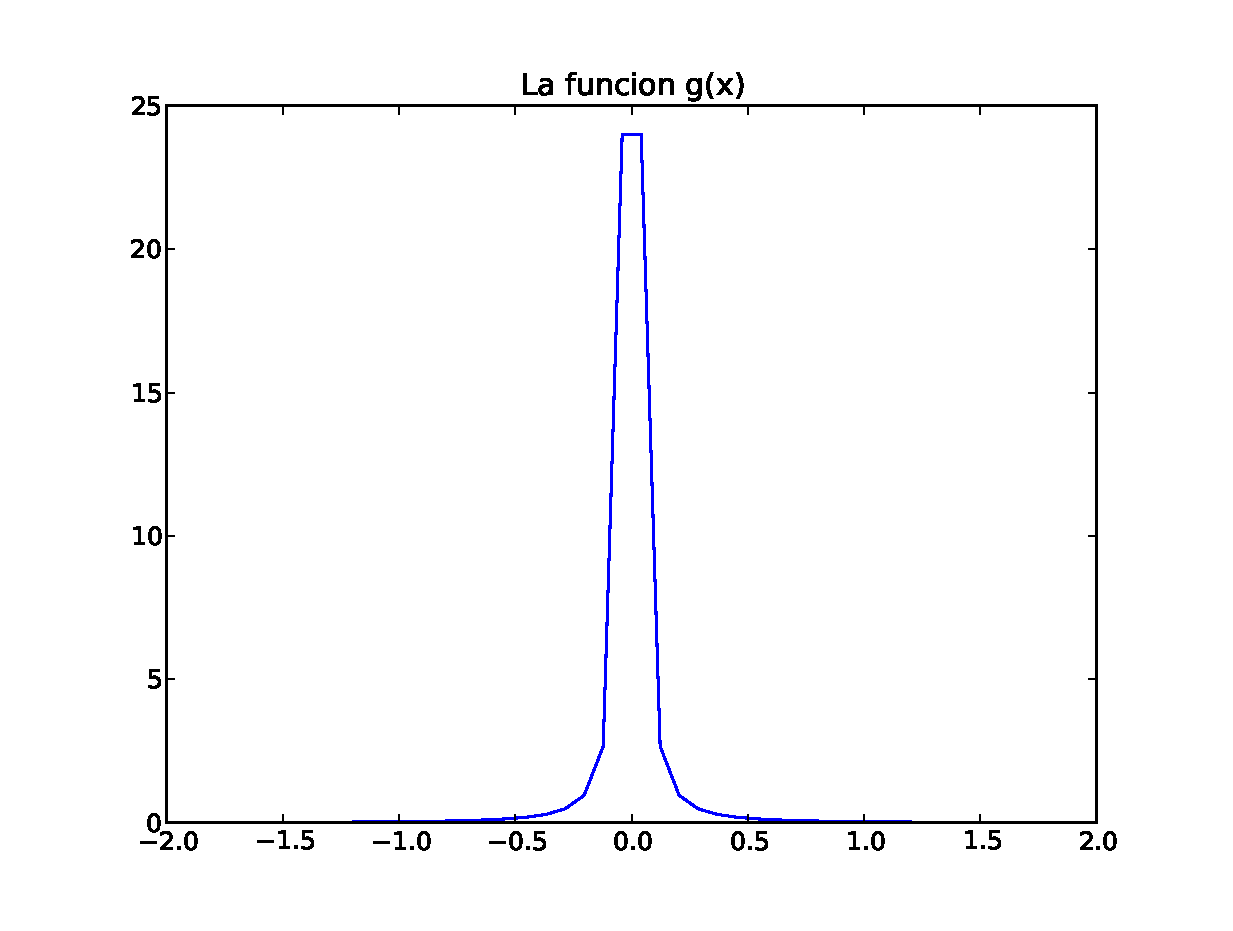
\includegraphics[scale=0.3]{Imagenes/grafica02.eps}  
\end{figure}
\end{minipage}
\end{frame}
\subsection{Consideración previa}
\begin{frame}
\frametitle{Consideración previa}
Antes de entrar de lleno a la revisión de las técnicas de interpolación, es necesario mencionar lo siguiente: dado que contamos con un conjunto finito de puntos, debemos de tener cuidado en el espaciamiento de la variable independiente.
\end{frame}
\begin{frame}
\frametitle{Consideración previa}
Si los puntos se alejan unos de otros, perderemos información para aquellos valores entre éstos puntos y la predicción de la interpolación ya no será la esperada.
\end{frame}
\begin{frame}
\frametitle{Ejemplo 3}
\fontsize{12}{12}\selectfont
Supongamos que tenemos seis mediciones como se indican en la siguiente figura, podemos ver claramente un comportamiento oscilatorio de la función, juzgando por los puntos y de acuerdo a las barras de error, una línea recta es la que probablemente nos ajustaría los puntos.
\begin{figure}
	\centering
	\includegraphics[scale=0.35]{Imagenes/figura01-1.eps} 
\end{figure}
\end{frame}
\begin{frame}
\frametitle{Gráfica de una interpolación}
Las técnicas de interpolación hacen lo que pidamos, pero no necesariamente son consistentes con un fenómeno o modelo.
\begin{figure}
	\centering
		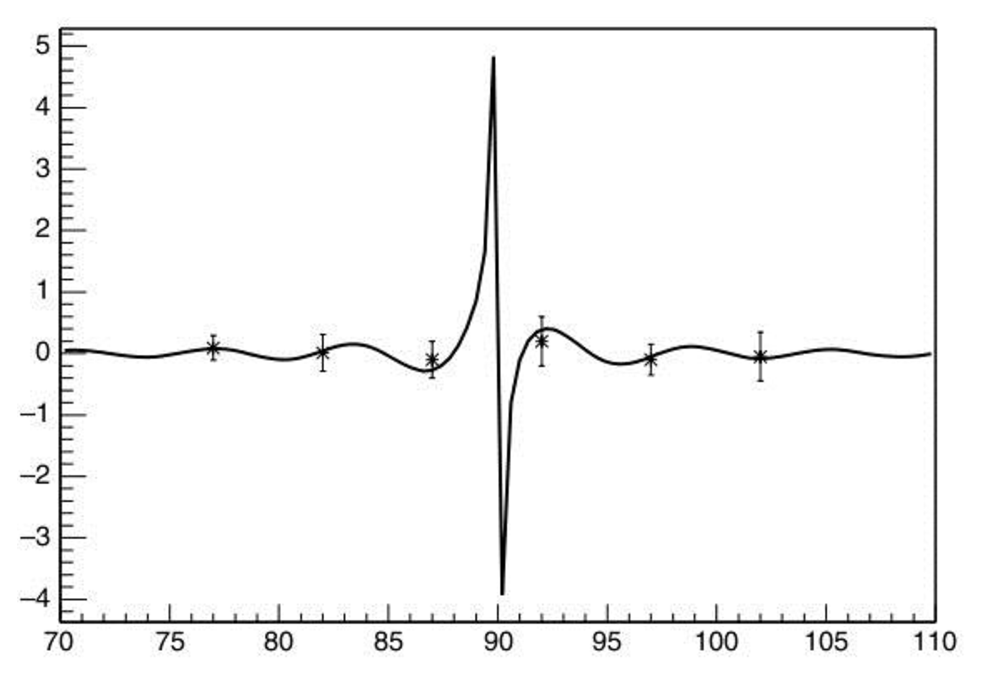
\includegraphics[scale=0.4]{Imagenes/figura02.eps} 
\end{figure}
\end{frame}
\section{Interpolación polinomial}
\frame{\tableofcontents[currentsection, hideothersubsections]}
\subsection{Interpolación de Lagrange}
\begin{frame}
\frametitle{Interpolación de Lagrange}
La técnica más sencilla de interpolación, es usando polinomios. Siempre es posible construir un \emph{único} polinomio de grado $n$ que pasa a través de $n + 1$ puntos.
\\
\medskip
Una manera de obtener este polinomio es usando la fórmula de Lagrange
\end{frame}
\begin{frame}
\frametitle{Fórmula de Lagrange}
\begin{equation}
P_{n}(x) = \sum_{i = 0}^{n} \: y_{i} \: \ell_{i}(x)
\label{eq:ecuacion_03_01a}
\end{equation}
donde $n$ es el grado del polinomio y
\begin{align}
\begin{aligned}
\ell_{i}(x) &= \dfrac{x - x_{0}}{x_{i} - x_{0}} \cdot \dfrac{x - x_{1}}{x_{i} - x_{1}} \ldots \dfrac{x - x_{i + 1}}{x_{i} - x_{i + 1}} \cdot \dfrac{x - x_{n}}{x_{i} - x_{n}} \\
 &= \prod_{\substack{j = 0 \\ j \neq i}}^{n} \; \dfrac{x - x_{j}}{x_{i} - x_{j}}, \hspace{0.5cm} i = 0,1,\ldots,n
\end{aligned}
\label{eq:ecuacion_03_01b}
\end{align}
se llaman \emph{funciones cardinales}.
\end{frame}
\begin{frame}
\frametitle{Por ejemplo, si $n = 1$}
La interpolación es una línea recta: 
\[P_{1}(x) = y_{0} \: \ell_{0}(x) + y_{1} \: \ell_{1}(x) \]
y las funciones cardinales son
\[ \ell_{0}(x) = \dfrac{x - x_{1}}{x_{0} - x_{1}} \hspace{1cm} \ell_{1}(x) = \dfrac{x - x_{0}}{x_{1} - x_{0}} \]
\end{frame}
\begin{frame}
\frametitle{Con $n = 2$}
La interpolación es parabólica:
\[P_{2}(x) = y_{0} \: \ell_{0}(x) + y_{1} \: \ell_{1}(x) + y_{2} \: \ell_{2}(x) \]
y las $\mathcal{L}_{i}(x)$ son:
\begin{eqnarray*}
\ell_{0}(x) &=& \dfrac{(x - x_{1})(x - x_{2})}{(x_{0} - x_{1})(x_{0} - x_{2})} \\
\ell_{1}(x) &=& \dfrac{(x - x_{0})(x - x_{2})}{(x_{1} - x_{0})(x_{1} - x_{2})} \\
\ell_{2}(x) &=& \dfrac{(x - x_{0})(x - x_{1})}{(x_{2} - x_{0})(x_{2} - x_{1})} 
\end{eqnarray*}
\end{frame}
\begin{frame}
\frametitle{Propiedad de las funciones cardinales}
Las funciones cardinales son polinomios de orden $n$ que tienen la propiedad
\begin{equation}
\ell_{i} (x_{j}) = \begin{cases} 0 \hspace{0.1cm} \mbox{si } i \neq j \\ 
1 \hspace{0.1cm} \mbox{si } i = j \end{cases} = \delta_{ij}
\label{eq:ecuacion_03_02}
\end{equation}
donde $\delta_{ij}$ es la delta de Kronecker.
\end{frame}
\begin{frame}
\frametitle{Fórmula de Lagrange}
Para probar que el polinomio de interpolación pasa por los puntos experimentales, sustituimos $x = x_{j}$ en la definición de $P_{n}(x)$ (ec. \ref{eq:ecuacion_03_01a}) y usamos la ec. (\ref{eq:ecuacion_03_02}, entonces:
\[ P_{n}(x_{j}) = \sum_{i = 0}^{n} y_{i} \: \ell_{i}(x_{j}) = \sum_{i = 0}^{n} y_{i} \: \delta_{ij} = y_{j} \]
\end{frame}
\begin{frame}
\frametitle{Error en la fórmula de Lagrange}
Se puede demostrar que el error en el polinomio de interpolación es
\[ f(x) - P_{n}(x) = \dfrac{(x - x_{0})(x - x_{1}) \ldots (x - x_{n})}{(n + 1)!} \: f^{(n+1)}(\xi)\]
donde $\xi \in (x_{0},x_{n})$, y éste valor normalmente no se conoce. 
\\
\bigskip
Debemos de notar que mientras más lejos están los datos de $x$, contribuye a que el error se incremente. 
\end{frame}
\subsubsection{Ejemplo}
\begin{frame}
\frametitle{Ejemplo}
Veamos el cambio de la presión del vapor de {}$^{4}$He como función de la temperatura, de acuerdo a la literatura tenemos que:
\fontsize{12}{12}\selectfont
\begin{center}
\begin{tabular}{c | l@{}}
Temperatura [K] & Presión de vapor [kPa] \\
\hline $2.3$ & $6.38512$ \\
\hline $2.7$ & $13.6218$ \\
\hline $2.9$ & $18.6760$ \\
\hline $3.2$ & $28.2599$ \\
\hline $3.5$ & $40.4082$ \\
\hline $3.7$ & $49.9945$
\end{tabular}
\end{center}
\end{frame}
\begin{frame}
\frametitle{Gráfica de los puntos experimentales}
\begin{figure}
	\centering
	\includegraphics[scale=0.4]{Imagenes/grafica03_1.eps}
	\caption{El conjunto de datos experimentales.}
\end{figure}
\end{frame}
\begin{frame}
\frametitle{Pregunta para resolver}
¿Cuál es el valor de presión a una temperatura de $\SI{3}{\kelvin}$?
\begin{figure}
	\centering
	\includegraphics[scale=0.4]{grafica03.eps} 
\end{figure}
\end{frame}
\begin{frame}[fragile]
\frametitle{Solución}
Tomamos lo que ya conocemos para $n=1$
\[P_{1}(x) = y_{0} \: \ell_{0}(x) + y_{1} \: \ell{1}(x) \]
\pause
y las funciones cardinales son
\[ \ell_{0}(x) = \dfrac{x - x_{1}}{x_{0} - x_{1}} \hspace{1cm} \ell_{1}(x) = \dfrac{x - x_{0}}{x_{1} - x_{0}} \]
\end{frame}
\begin{frame}[fragile]
\frametitle{Solución}
En nuestro ejemplo, tenemos que:
\begin{align*}
(x_{0}, y_{0}) = (2.9, 18.6760) \\
\\
(x_{1}, y_{1}) = (3.2, 28.2599)
\end{align*}
\visible<2->{Con la interpolación lineal, tenemos que para una temperatura de \textcolor{blue}{$\SI{3.0}{\kelvin}$}, la presión tiene un valor de \textcolor{red}{$\mathbf{\SI{21.87}{\kilo\pascal}}$}}
\end{frame}
\begin{frame}
\frametitle{Interpolación cuadrática}
Con la intención de mejorar nuestro resultado, podemos usar un polinomio de segundo orden, es decir $n = 2$
\[P_{2}(x) = y_{0} \: \ell_{0}(x) + y_{1} \: \ell_{1}(x) + y_{2} \: \ell_{2}(x) \]
\end{frame}
\begin{frame}
\frametitle{Interpolación cuadrática}
Las funciones cardinales $\ell_{i}(x)$ son:
\begin{align*}
\ell_{0}(x) &= \dfrac{(x - x_{1})(x - x_{2})}{(x_{0} - x_{1})(x_{0} - x_{2})} \\
\\
\ell_{1}(x) &= \dfrac{(x - x_{0})(x - x_{2})}{(x_{1} - x_{0})(x_{1} - x_{2})} \\
\\
\ell_{2}(x) &= \dfrac{(x - x_{0})(x - x_{1})}{(x_{2} - x_{0})(x_{2} - x_{1})} 
\end{align*}
\end{frame}
\begin{frame}
\frametitle{Usando los datos experimentales}
Usando los valores de la tabla anterior:
\begin{eqnarray*}
(x_{0}, y_{0}) = (2.7, 13.6218) \\
(x_{1}, y_{1}) = (2.9, 18.6760) \\
(x_{2}, y_{2}) = (3.2, 28.2599)
\end{eqnarray*}
\visible<2->{A una temperatura de \textcolor{blue}{$\SI{3.0}{\kelvin}$}, la presión de vapor tiene un valor de \textcolor{red}{$\mathbf{\SI{21.671}{\kilo\pascal}}$}}
\\
\bigskip
\visible<3->{El siguiente paso es usar cuatro puntos y construir el polinomio de orden $3$.}
\end{frame}
\begin{frame}
\frametitle{Ejercicio}
\begin{minipage}{5cm}
A partir de la siguiente tabla de datos,
\\
\medskip
\begin{center}
\begin{tabular}{c | c}
x & P(x) \\
\hline $1$ & $0.671$ \\
\hline $2$ & $0.620$ \\
\hline $3$ & $0.567$ \\
\hline $4$ & $0.512$
\end{tabular}
\end{center}
\end{minipage}
\hspace{0.3cm}
\visible<2->{
\begin{minipage}{5cm}
\fontsize{12}{12}\selectfont
Usa el algoritmo de interpolación de Lagrange con un polinomio de grado $n = 3$, para estimar el valor de $P(x)$ en los siguientes puntos:
\\
\medskip
$x= 1.5,2.5, 3.5$
\end{minipage}}
\end{frame}
\begin{frame}[allowframebreaks, fragile]
\frametitle{Solución al problema}
\begin{lstlisting}[caption=Código para la interpolación de Lagrange,style= FormattedNumber, basicstyle=\linespread{0.9}\ttfamily\small, columns=fullflexible]
import numpy as np
n = 3
x_0_ = np.array([1.5, 2.5, 3.5])
x = np.array([1., 2., 3., 4.])
f = np.array([0.671, 0.620, 0.567, 0.512])

for k in x_0_:
    yres = 0
    for i in range(0, n + 1):
        z = 1.0
        for j in range(0, n + 1):
            if i != j:
                z = z * (k - x[j])/(x[i] - x[j])
        yres = yres + z*f[i]
    
    print ('El polinomio evaluado en P(',k,') =',  yres)
\end{lstlisting}
\end{frame}
\begin{frame}[fragile]
\frametitle{Solución (en la terminal y con una gráfica)}
%\begin{minipage}{5cm}
\begin{center}
\begin{tabular}{c | l}
x & P(x) \\
\hline $1$   & $0.671$ \\
\hline $1.5$ & $0.64575$ \\
\hline $2$   & $0.620$ \\
\hline $2.5$ & $0.59375$ \\
\hline $3$   & $0.567$ \\
\hline $3.5$ & $0.53975$ \\
\hline $4$   & $0.512$
\end{tabular}
\end{center}
%\end{minipage}
\end{frame}
\begin{frame}
\frametitle{Solución con una gráfica}
\begin{figure}
	\centering
	\includegraphics[scale=0.5]{Imagenes/InterpLagrangen3_01.eps}
	\caption{Gráfica con los datos experimentales}
\end{figure}
\end{frame}
\begin{frame}
\frametitle{Solución con una gráfica}
\begin{figure}
	\centering
	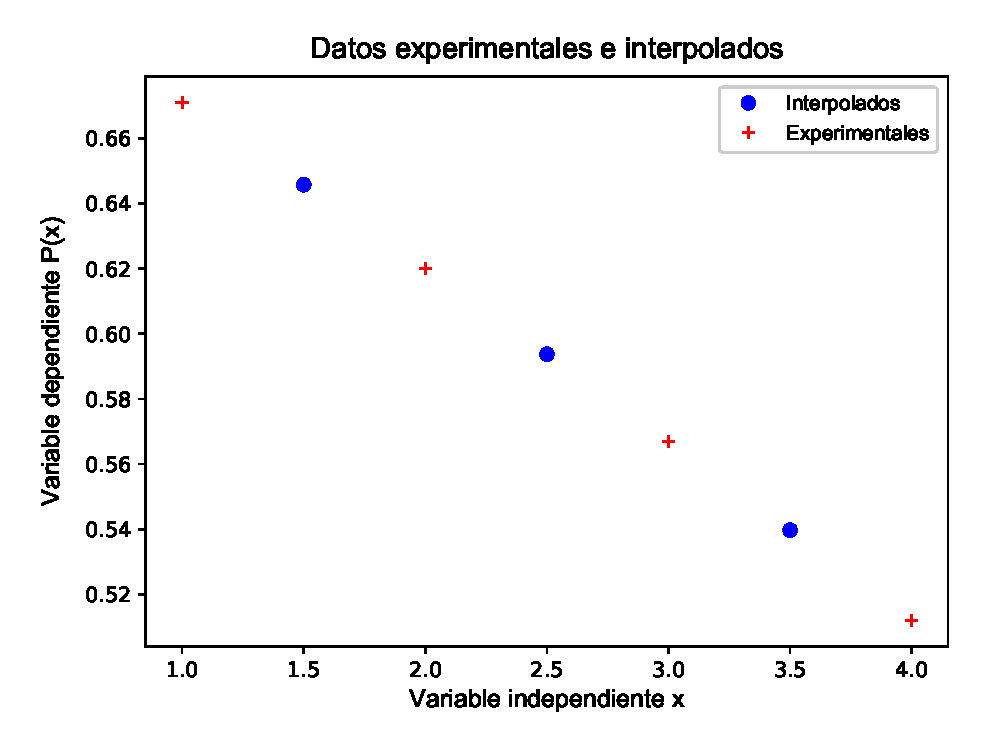
\includegraphics[scale=0.5]{Imagenes/InterpLagrangen3_02.eps}
	\caption{Gráfica con los datos experimentales y el valor de interpolación -bola azul-}
\end{figure}
\end{frame}
\subsection{Ejercicios}
\begin{frame}
\frametitle{Ejercicios}
\setbeamercolor{item projected}{bg=green!70!black,fg=white}
\setbeamertemplate{enumerate items}[circle]
\begin{enumerate}
\item Ajusta $x \sin(x$) en $[0, \pi/2]$ con un polinomio de interpolación de Lagrange de orden $n = 4$, utilizando puntos con igual separación.
\\
\bigskip
Calcula el error de cada interpolación en cada incremento de $\pi/16$, muestra una gráfica.
\seti
\end{enumerate}
\end{frame}
\begin{frame}
\frametitle{Ejercicios}
\setbeamercolor{item projected}{bg=green!70!black,fg=white}
\setbeamertemplate{enumerate items}[circle]
\begin{enumerate}
\conti
\item Ajusta $\sin(x)$ en $[0, 2\pi]$ con el polinomio de interpolación de Lagrange de orden $n = 4$ y $n = 8$, utilizando puntos con igual separación ($5$ y $9$ puntos respectivamente). 
\\
\bigskip
Grafica los polinomios de interpolación junto con $\sin(x)$ y las distribuciones de sus errores.
\end{enumerate}
\end{frame}
\begin{frame}[fragile]
\frametitle{Hints para resolver los ejercicios}
Tomemos en cuenta los siguiente:
\setbeamercolor{item projected}{bg=green!70!black,fg=white}
\setbeamertemplate{enumerate items}[circle]
\begin{enumerate}[<+->]
\item Hay que dividir el intervalo $[0,\pi/2]$ con cinco espacios.
\item Se evalúa la función $x \: sin(x)$ en el conjunto de puntos que obtuvimos.
\item Creamos un conjunto de puntos para ajustar con el método de Lagrange.
\item La manera más fácil es con un \texttt{linspace}.
\end{enumerate}
\end{frame}
%\begin{frame}[fragile]
%\frametitle{Obteniendo los datos para el ejercicio}
%\begin{lstlisting}
%n=4
%x0 = linspace(0.,pi/2,20)
%x = linspace(0.,pi/2,5)
%f = funcion(x)
%calculo=[]
%\end{lstlisting}
%\end{frame}
%\begin{frame}[fragile]
%\frametitle{Función f(x)}
%\begin{lstlisting}
%def funcion(x):
%    return x*sin(x)
%\end{lstlisting}
%\end{frame}
%\begin{frame}[fragile]
%\frametitle{Método de Lagrange}
%\begin{lstlisting}
%def metLagrange(n,x0,x):
%    for k in x0:
%        yres = 0
%        for i in range(0,n+1):
%            z = 1.0
%            for j in range(0,n+1):
%                if i != j:
%                    z = z * (k-x[j])/(x[i]-x[j])
%            yres = yres + z*f[i]
%        calculo.append(yres)        
%\end{lstlisting}
%\end{frame}
\begin{frame}
\frametitle{Solución Ejercicio 1}
\begin{figure}
	\centering
	\includegraphics[scale=0.45]{Imagenes/ejercicioTema21_1.eps} 
\end{figure}
\end{frame}
\begin{frame}
\frametitle{Solución Ejercicio 2}
\begin{figure}
	\centering
	\includegraphics[scale=0.45]{Imagenes/ejercicioTema21_2.eps} 
\end{figure}
\end{frame}
\section{Consideraciones importantes}
\subsection{Consideraciones importantes}
\begin{frame}
\frametitle{Consideraciones importantes}
La técnica de interpolación de Lagrange supone que el espaciamiento entre los puntos es la misma, por lo que cuando se presentan puntos que no cumplen ésta condición, la técnica ya no aplicaría.
\end{frame}
\subsection{Desventajas interpolación de Lagrange}
\begin{frame}
\frametitle{Desventajas interpolación de Lagrange}
A continuación se presentan algunas de las desventajas de la primera técnica de interpolación, al interpolación de Lagrange que hemos estudiado.
\end{frame}
\begin{frame}
\frametitle{Desventajas interpolación Lagrange}
\begin{itemize}[<+->]
\item [\textcolor{red}{\xmark}] La cantidad de cálculos necesarios para una interpolación es grande.
\item [\textcolor{red}{\xmark}] La interpolación para otro valor de $x$ necesita la misma cantidad de cálculos adicionales, ya que no se pueden utilizar partes de la aplicación previa.
\end{itemize}
\end{frame}
\begin{frame}
\frametitle{Desventajas interpolación Lagrange}
\begin{itemize}[<+->]
\item [\textcolor{red}{\xmark}] Cuando el número de datos tiene que incrementarse o decrementarse, no se pueden utilizar los resultados de los cálculos previos.
\item [\textcolor{red}{\xmark}] La evaluación del error no es fácil.
\end{itemize}
\end{frame}
\section{Interpolación de Newton}
\frame{\tableofcontents[currentsection, hideothersubsections]}
\subsection{Definición}
\begin{frame}
\frametitle{Interpolación de Newton}
Aunque el método de interpolación de Lagrange es conceptualmente sencillo, no es en sí, un algoritmo eficiente.
\\
\medskip
Un mejor método computacional se obtiene con el \textoazul{Método de Newton}.
\end{frame}
\begin{frame}
\frametitle{Interpolación de Newton}
El polinomio de interpolación de Newton se escribe de la forma:
\fontsize{12}{12}\selectfont
\[ \begin{split}
P_{n}(x) = a_{0} + (x - x_{0}) \: a_{1} + (x - x_{0})(x - x_{1}) \: a_{2} + \ldots + \\
+ (x - x_{0})(x - x_{1}) \ldots (x - x_{n - 1}) \: a_{n} 
\end{split} \]
\fontsize{14}{14}\selectfont
\pause
Este polinomio nos permite contar con un procedimiento de evaluación más eficiente.
\end{frame}
\begin{frame}
\frametitle{Evaluación más eficiente}
Por ejemplo, con cuatro pares de datos ($n = 3$), tenemos que el polinomio de interpolación de Newton es:
\begin{align*}
P_{3}(x) =& a_{0} + (x - x_{0}) \: a_{1} (x - x_{0})(x - x_{1}) \: a_{2} + \\		
{}& \hspace*{1cm} + (x - x_{0})(x - x_{1})(x - x_{2}) \: a_{3}  \\
\\
P_{3}(x) =& a_{0} + \left\lbrace a_{1}+(x-x_{1})\left[a_{2}+(x-x_{2})a_{3} \right] \right\rbrace 
\end{align*}
\end{frame}
\begin{frame}
\frametitle{Evaluación del polinomio}
\begin{align*}
P_{3}(x) = a_{0} + \left\lbrace a_{1}+(x-x_{1})\left[a_{2}+(x-x_{2})a_{3} \right] \right\rbrace 
\end{align*}
Que puede ser evaluado hacia atrás con las siguientes relaciones de recurrencia:
\begin{eqnarray*}
P_{0} &=& a_{3} \\
P_{1} &=& a_{2} + (x - x_{2}) \: P_{0}(x) \\
P_{2} &=& a_{1} + (x - x_{1}) \: P_{1}(x) \\
P_{3} &=& a_{0} + (x - x_{0}) \: P_{2}(x) 
\end{eqnarray*}
\end{frame}
\begin{frame}
\frametitle{Evaluación del polinomio}
\visible<2->{Para un $n$ arbitrario, tenemos:}
\visible<3->{
\begin{align}
\begin{aligned}
P_{0}(x) =& \: a_{n} \\
P_{k} =& \: a_{n - k} + (x - x_{n - k}) \: P_{k - 1}(x), \hspace{0.5cm} k = 1,2,\ldots,n
\end{aligned}
\label{eq:ecuacion_03_04}
\end{align}
}
\end{frame}
\begin{frame}[fragile]
\frametitle{Estructurando el código en \python}
Definimos \texttt{xDatos} para las coordenadas $x$ del conjunto de puntos y $n$ al grado de polinomio, podemos usar el siguiente algoritmo para calcular $P_{n}(x)$:
\begin{lstlisting}[caption=Nombre Codigo, style=FormattedNumber, basicstyle=\linespread{1.1}\ttfamily=\small, columns=fullflexible]
p = a[n]
for k in range(1, n + 1):
    p = a[n-k] + (x - xDatos[n-k]) * p
\end{lstlisting}
\end{frame}
\begin{frame}
\frametitle{Coeficientes del polinomio}
Los coeficientes de $P_{n}$ se calculan forzando que el polinomio pase a través del conjunto de puntos $y_{i}=P_{n}(x_{i}),\hspace{0.5cm} i =0,1,\ldots,n$. 
\end{frame}
\begin{frame}
\frametitle{Coeficientes del polinomio}
De tal manera que tenemos un sistema de ecuaciones simultáneas:
\begin{align*}
y_{0} &= a_{0} \\
y_{1} &= a_{0} + (x_{1} - x_{0}) \: a_{1} \\
y_{2} &= a_{0} + (x_{2} - x_{0}) \: a_{1} + (x_{2} - x_{0})(x_{2} - x_{1}) \: a_{2} \\
\vdots \\
y_{n} &= a_{0} + (x_{n} - x_{0}) \: a_{1} + \ldots + \\
       &+ (x_{n} - x_{0})(x_{n} - x_{1}) \ldots (x_{n} - x_{n - 1}) \: a_{n}
\end{align*}
\end{frame}
\subsection{Diferencias divididas}
\begin{frame}[fragile]
\frametitle{Diferencias divididas}
Se introducen las diferencias divididas, de la siguiente forma:
\begin{eqnarray*}
\nabla y_{i} &=& \dfrac{y_{i} - y_{0}}{x_{i} - x_{0}}, \hspace{1cm} i = 1,2,\ldots,n \\
\visible<2->{\nabla^{2} y_{i} &=& \dfrac{\nabla y_{i} - \nabla y_{1}}{x_{i} - x_{1}}, \hspace{1cm} i = 1,2,\ldots,n} \\
\visible<3->{\nabla^{3} y_{i} &=& \dfrac{\nabla^{2} y_{i} - \nabla^{2} y_{2}}{x_{i} - x_{2}}, \hspace{1cm} i = 1,2,\ldots,n} \\
\visible<4->{\vdots} \\
\visible<5->{\nabla^{n} y_{i} &=& \dfrac{\nabla^{n-1} y_{n} - \nabla^{n-1} y_{n-1}}{x_{n} - x_{n-1}}}
\end{eqnarray*}
\end{frame}
\begin{frame}
\frametitle{Diferencias divididas}
La solución al sistema de ecuaciones es:
\begin{eqnarray*}
a_{0} &=& y_{0} \\
a_{1} &=& \nabla y_{1} \\
a_{2} &=& \nabla^{2} y_{2} \\
\vdots \\
a_{n} &=& \nabla^{n} y_{n}
\end{eqnarray*}
\end{frame}
\begin{frame}
\frametitle{Diferencias divididas}
Si los coeficientes se calculan a mano, es convieniente escribirlos con el siguiente formato:
(con $n=4$)
\\
\medskip
\begin{center}
\begin{tabular}{| c | c | c | c | c | c |}
\hline $x_{0}$ & $y_{0}$ & & & & \\
\hline $x_{1}$ & $y_{1}$ & $\nabla y_{1}$ & & & \\
\hline $x_{2}$ & $y_{2}$ & $\nabla y_{2}$ & $\nabla^{2} y_{2}$ & &  \\
\hline $x_{3}$ & $y_{3}$ & $\nabla y_{3}$ & $\nabla^{2} y_{3}$ & $\nabla^{3} y_{3}$ &  \\
\hline $x_{4}$ & $y_{4}$ & $\nabla y_{4}$ & $\nabla^{2} y_{4}$ & $\nabla^{3} y_{4}$ & $\nabla^{4} y_{4}$ \\
\hline
\end{tabular}
\end{center}
\end{frame}
\begin{frame}
\frametitle{Diferencias divididas}
\textoazul{Los términos en la diagonal}
\[ (y_{0}, \nabla y_{1}, \nabla^{2} y_{2}, \nabla^{3} y_{3}, \nabla^{4} y_{4}) \]
\pause
\textoazul{son los coeficientes del polinomio}.
\end{frame}
\begin{frame}
\frametitle{Diferencias divididas}
Si los puntos de datos se enumeran en un orden diferente, las entradas de la tabla van a cambiar, pero el polinomio resultante será el mismo.
\\
\bigskip
Recordemos que un polinomio de interpolación de grado $n$ con $n + 1$ datos diferentes, es único.
\end{frame}
\begin{frame}[fragile]
\frametitle{Estructurando el código}
Las operaciones en la computadora se pueden realizar con un arreglo unidimensional $a$, usando el siguiente algoritmo (tomando la notación $m = n + 1$ = número de puntos):
\end{frame}
\begin{frame}[fragile]
\frametitle{Estructurando el código}
\begin{lstlisting}[caption=Calculando los coeficientes del polinomio, style=FormattedNumber, basicstyle=\linespread{1.1}\ttfamily=\small, columns=fullflexible]
a = yDatos.copy()
for k in range(1, m):
    for i in range(k, m):
        a[i] = (a[i] - a[k-_1_])/(xDatos[i] - xDatos[k-_1_])
\end{lstlisting}
\end{frame}
\begin{frame}
\frametitle{Estructurando el código}
Inicialmente el arreglo $a$ contiene las coordenadas $y$ del conjunto de datos, es decir, la segunda columna de la tabla.
\end{frame}
\begin{frame}
\frametitle{Estructurando el código}
Cada vez que pasa por el bucle externo, se genera la siguiente columna, por lo que se sobre-escriben los elementos de $a$, por tanto, al concluir el bucle, $a$ contiene los elementos de la diagonal, que son los coeficientes del polinomio.
\end{frame}
\subsection{Módulos propios de interpolación con \python}
\begin{frame}
\frametitle{Módulos propios de interpolación con \python}
Para facilitar el mantenimiento y la lectura cuando los programas son demasiado largos, es posible \enquote{dividirlos} en \textcolor{blue}{módulos}, agrupando elementos relacionados.
\end{frame}
\subsection{Módulo \texttt{newtonPoli}}
\begin{frame}
\frametitle{Módulo \texttt{newtonPoli}}
El módulo \funcionazul{newtonPoli} incluye dos funciones que se requieren para la interpolación de Newton.
\setbeamercolor{item projected}{bg=green!70!black,fg=white}
\setbeamertemplate{enumerate items}[circle]
\begin{enumerate}[<+->]
\item La función \funcionazul{coeffts}.
\item La función \funcionazul{evalPoli}
\end{enumerate}
\end{frame}
\begin{frame}
\frametitle{La función \funcionazul{coeffts}}
Dados el conjuntos de puntos en los arreglos \texttt{xDatos} y \texttt{yDatos}, la función \funcionazul{coeffts} devuelve el arreglo $a$ con los coeficientes.
\end{frame}
\begin{frame}
\frametitle{La función \funcionazul{evalPoli}}
Una vez que ya conocemos los coeficientes, el polinomio $P_{n}(x)$ puede evaluarse para cualquier valor de $x$ con la función \funcionazul{evalPoli}.
\end{frame}
\begin{frame}[fragile]
\frametitle{Código del módulo}
\begin{lstlisting}[caption=Funciones \texttt{coeffts} del módulo \texttt{newtonPoli}, style=FormattedNumber, basicstyle=\linespread{1.1}\ttfamily=\small, columns=fullflexible]    
def coeffts(xDatos, yDatos):
    m = len(xDatos) 
    a = yDatos.copy()
    for k in range(1, m):
        a[k:m] = (a[k:m] - a[k-1])/(xDatos[k:m] - xDatos[k-1])
    return a
\end{lstlisting}
\end{frame}
\begin{frame}[fragile]
\frametitle{Código del módulo}
\begin{lstlisting}[caption=Funciones \texttt{evalPoli} del módulo \texttt{newtonPoli}, style=FormattedNumber, basicstyle=\linespread{1.1}\ttfamily=\small, columns=fullflexible]
def evalPoli(a, xDatos, x):
    n = len(xDatos) - 1 
    p = a[n]
    for k in range(1, n+1):
        p = a[n-k] + (x - xDatos[n-k]) * p
    return p
\end{lstlisting}
\end{frame}
\begin{frame}
\frametitle{Ejemplo}
Los datos que se muestran en la siguiente tabla:
\begin{table}[htbp]
\centering \small
\begin{tabulary}{15cm}{c | c | c | c | c | c | c}
$x$ & $0.15$ & $2.30$ & $3.15$ & $4.85$ & $6.25$ & $7.95$ \\
\midrule $y$ & $4.79867$ & $4.49013$ & $4.2243$ & $3.47313$ & $2.66674$ & $1.51909$
\end{tabulary}
\end{table}
Se obtuvieron de la función
\[ f(x) = 4.8 \: \cos \left( \dfrac{\pi \: x}{20} \right)\]
\end{frame}
\begin{frame}
\frametitle{Ejemplo}
Con ese conjunto de datos, interpola mediante el polinomio de Newton en
\[ x=0, 0.5, 1.0, 1.5, \ldots,7.5, 8.0 \]
\\
\bigskip
Compara los resultados con el valor \enquote{exacto} de los valores $y_{i} = f(x_{i})$
\end{frame}
\begin{frame}[fragile]
\frametitle{Solución al ejemplo}
¿Qué necesitamos?
\\
\bigskip
Abriendo un archivo en Spyder, llamamos a la librería \funcionazul{numpy} y también al módulo \funcionazul{newtonPoli} que contiene las funciones para resolver el polinomio de interpolación:
\end{frame}
\begin{frame}[fragile]
\frametitle{Llamada a las librerías}
\begin{lstlisting}[caption=Llamando a las librerías y módulos, style=FormattedNumber, basicstyle=\linespread{1.1}\ttfamily=\small, columns=fullflexible]
from numpy import *
from newtonPoli import *
\end{lstlisting}
\end{frame}
\begin{frame}[fragile]
\frametitle{Definiendo los arreglos}
Hay que crear los arreglos \texttt{xDatos} y \texttt{yDatos}, el arreglo $a$ se obtiene de la función \funcionazul{coeffts}.
\begin{lstlisting}[caption=Nombre Codigo, style=FormattedNumber, basicstyle=\linespread{1.1}\ttfamily=\small, columns=fullflexible]
xDatos = array([0.15,2.3,...,7.95])

yDatos = array([4.79867,4.49013,...,1.51909])

a = coeffts(xDatos, yDatos)
\end{lstlisting}
\end{frame}
\begin{frame}[fragile]
\frametitle{Evaluación de los puntos}
La siguiente parte es proporcionar el rango de puntos en donde queremos evaluar mediante el método de Newton, a través de la función \funcionazul{evalPoli}:
\end{frame}
\begin{frame}[fragile]
\frametitle{Evaluación de los puntos}
\begin{lstlisting}[caption=Evaluando los puntos y el error relativo, style=FormattedNumber, basicstyle=\linespread{1.1}\ttfamily=\small, columns=fullflexible]
for x in arange(0.0, 8.1, 0.5):
    y = evalPoli(a, xDatos, x)
    yExacta = 4.8 * cos(pi * x/20.0)
    print ('{:1.1f} \t {:1.5f} \t {:1.5f} \t {:1.5E}'.format(x, y, yExacta, errorRelativo(yExacta, y)))
\end{lstlisting}
\begin{lstlisting}
\end{lstlisting}
\end{frame}
\begin{frame}
Al ejecutar el código obtenemos lo siguiente:
\fontsize{12}{12}\selectfont
\begin{center}
\begin{tabular}{l l l l}
x & yInterp & yExacta & erroRelativo\\
%\multicolumn{4}{l}{----------------------------------------} \\
$0.0$ & $4.80003$ & $4.80000$ & $5.22802E-04$ \\
$0.5$ & $4.78518$ & $4.78520$ & $5.16392E-04$ \\
$1.0$ & $4.74088$ & $4.74090$ & $5.70846E-04$ \\
$1.5$ & $4.66736$ & $4.66738$ & $3.19661E-04$ \\
\vdots \\
$7.0$ & $2.17915$ & $2.17915$ & $3.43797E-04$ \\
$7.5$ & $1.83687$ & $1.83688$ & $6.76648E-04$ \\
$8.0$ & $1.48329$ & $1.48328$ & $2.67576E-04$
\end{tabular}
\end{center}
\end{frame}
\begin{frame}
\frametitle{Graficando la función exacta y los puntos}
\begin{figure}
	\centering
	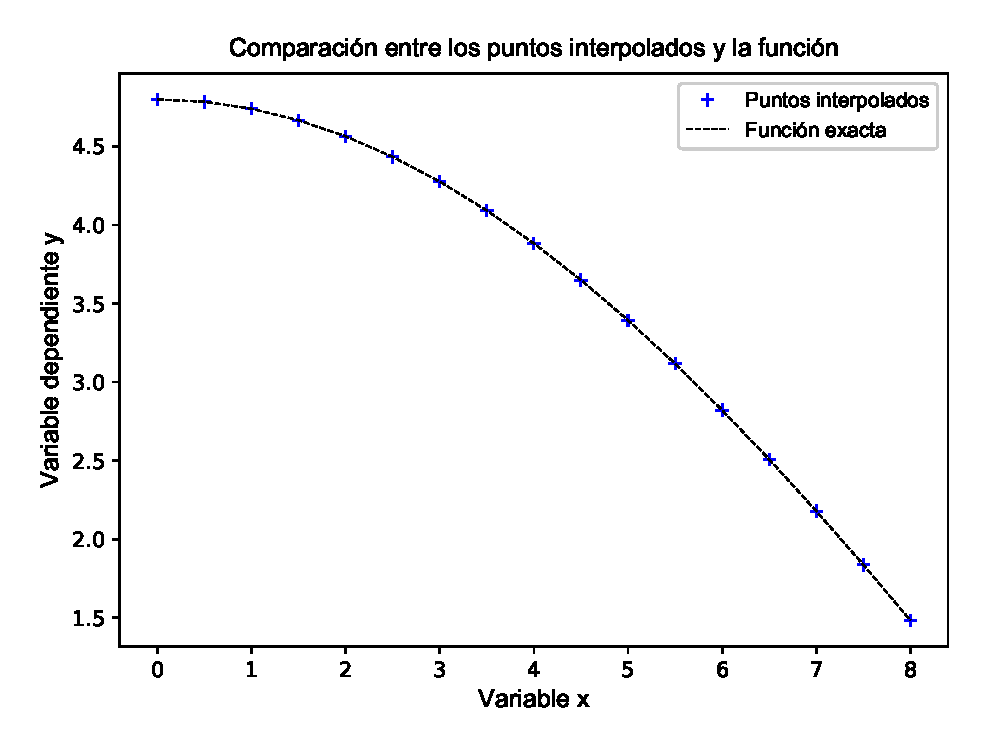
\includegraphics[scale=0.5]{EjemploInterpNewton_01.eps}
	\caption{Gráfica donde se visualizan los datos interpolados y la función.}
\end{figure}
\end{frame}
\end{document}